\section{Introduction}

Machine Learning (ML) is revolutionizing many fields.
It is now being used in a diverse range of domains including e-commerce, web and social media, interactive agents, and even in critical applications in autonomous vehicles and healthcare.
From a software systems point of view, ML can be viewed as a flexible framework for \textit{programming the unprogrammable}.
For instance, it is nearly impossible for a software engineer to program an object detector that can identify different objects in an image.
But using ML and a sufficient amount of labeled training data one can \textit{learn a program} to do the same that can even surpass human-level accuracy.

Database management systems (DBMSs) are complex software systems, that are the result of decades of research and complex software development.
They are at the core of many critical software applications and have also influenced much of the development of other popular data management systems such as NoSQL, Big Data, and Machine Learning Systems.
Out of the many types of database management systems, relational database management systems remains the most widely used type.
Thus for this paper, we primarily focus on relational database management systems.

DBMSs are also full of really-hard unprogrammable problems such as query optimization, physical database design optimization, and buffer management.
These problems are unprogrammable either because they have interactable search spaces and/or due to the inability to know what is going to happen next and hence cannot develop a program to find the optimal solution.
As a result, DBMS developers have to resort to using heuristics (and/or solution space restrictions) in order to solve these problems.
The goal of these heuristics is not to find an optimal solution for a specific instance but to find a solution which is not bad for all instances.

In this paper, we survey the existing landscape of using ML to program the programmable in DBMSs. 
We divide the DBMS into three main sub-components: 1) Query Parser, 2) Relational Engine, 3) Execution Engine, and identify several systems that incorporate ML into optimizing these sub-components. 
We also present several overarching design decisions that one has to make when integrating ML-based components into a DBMS and the trade-offs of available options.
Finally, we identify several open challenges that bottleneck the practical adoption of ML in DBMS internals.
The table provides a summary of this survey.

\begin{figure*}
    \centering
    \vspace{-6mm}
    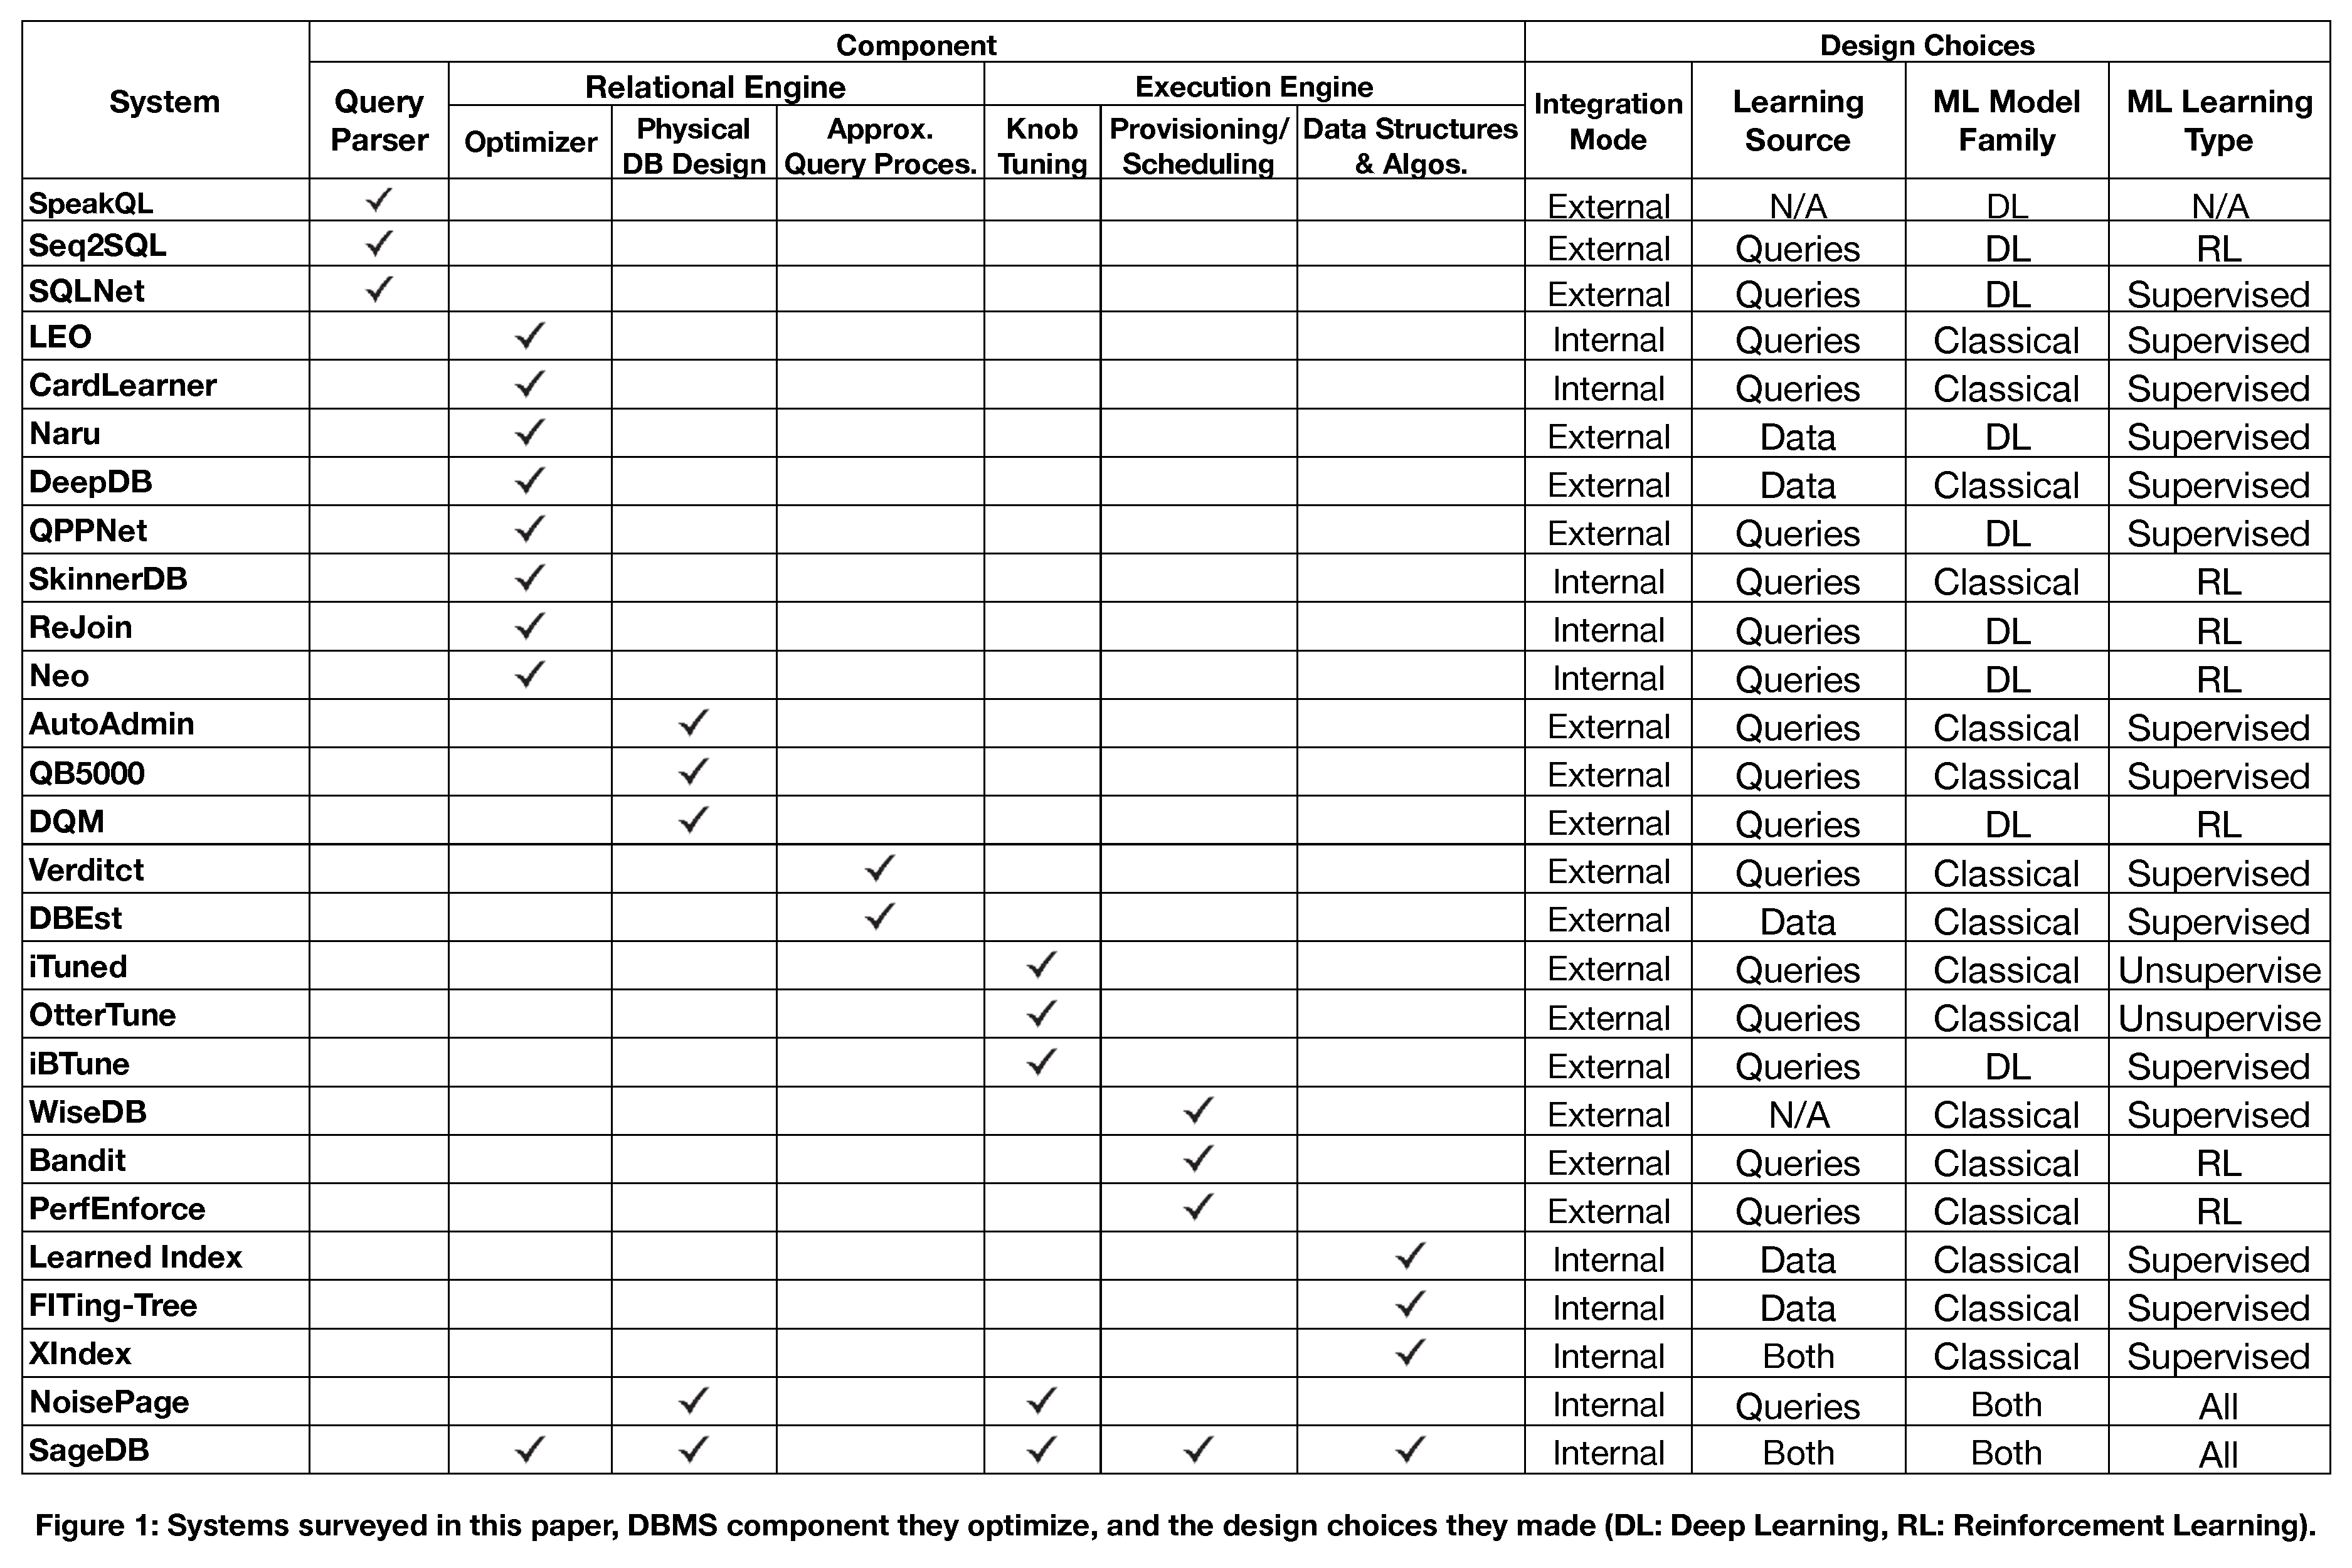
\includegraphics[height=0.85\textwidth, angle=90]{images/taxonomy.pdf}
\end{figure*}

The rest of this paper is organized as follows.
Section 2 provides some background on ML methods and DBMS internal in order to understand the rest of this paper.
Section 3, 4, and 5 present the use of ML in Query Parser, Relational Engine, and Execution Engine, respectively.
Section 6 presents the design choices and Section 7 presents the open-challenges.
We give our concluding remarks in Section 8.